\section{\Wilds datasets}
\label{sec:datasets}
We now briefly describe each \Wilds dataset, as summarized in \reffig{datasets}.
For each dataset, we consider a problem setting---domain generalization, subpopulation shift, or a hybrid---that we believe best reflects the real-world challenges in the corresponding application area; see \refapp{app_realism} for more discussion of these considerations.
To avoid confusion between our modified datasets and their original sources,
we append \textsc{\suffix{}} to the dataset names.
We provide more details and context on related distribution shifts for each dataset in \refapp{app_datasets}.

\subsection{Domain generalization datasets}

\subsubsection{\iWildCam: Species classification across different camera traps}\label{sec:dataset_iwildcam}

\begin{figure}[h!]
  \centering
  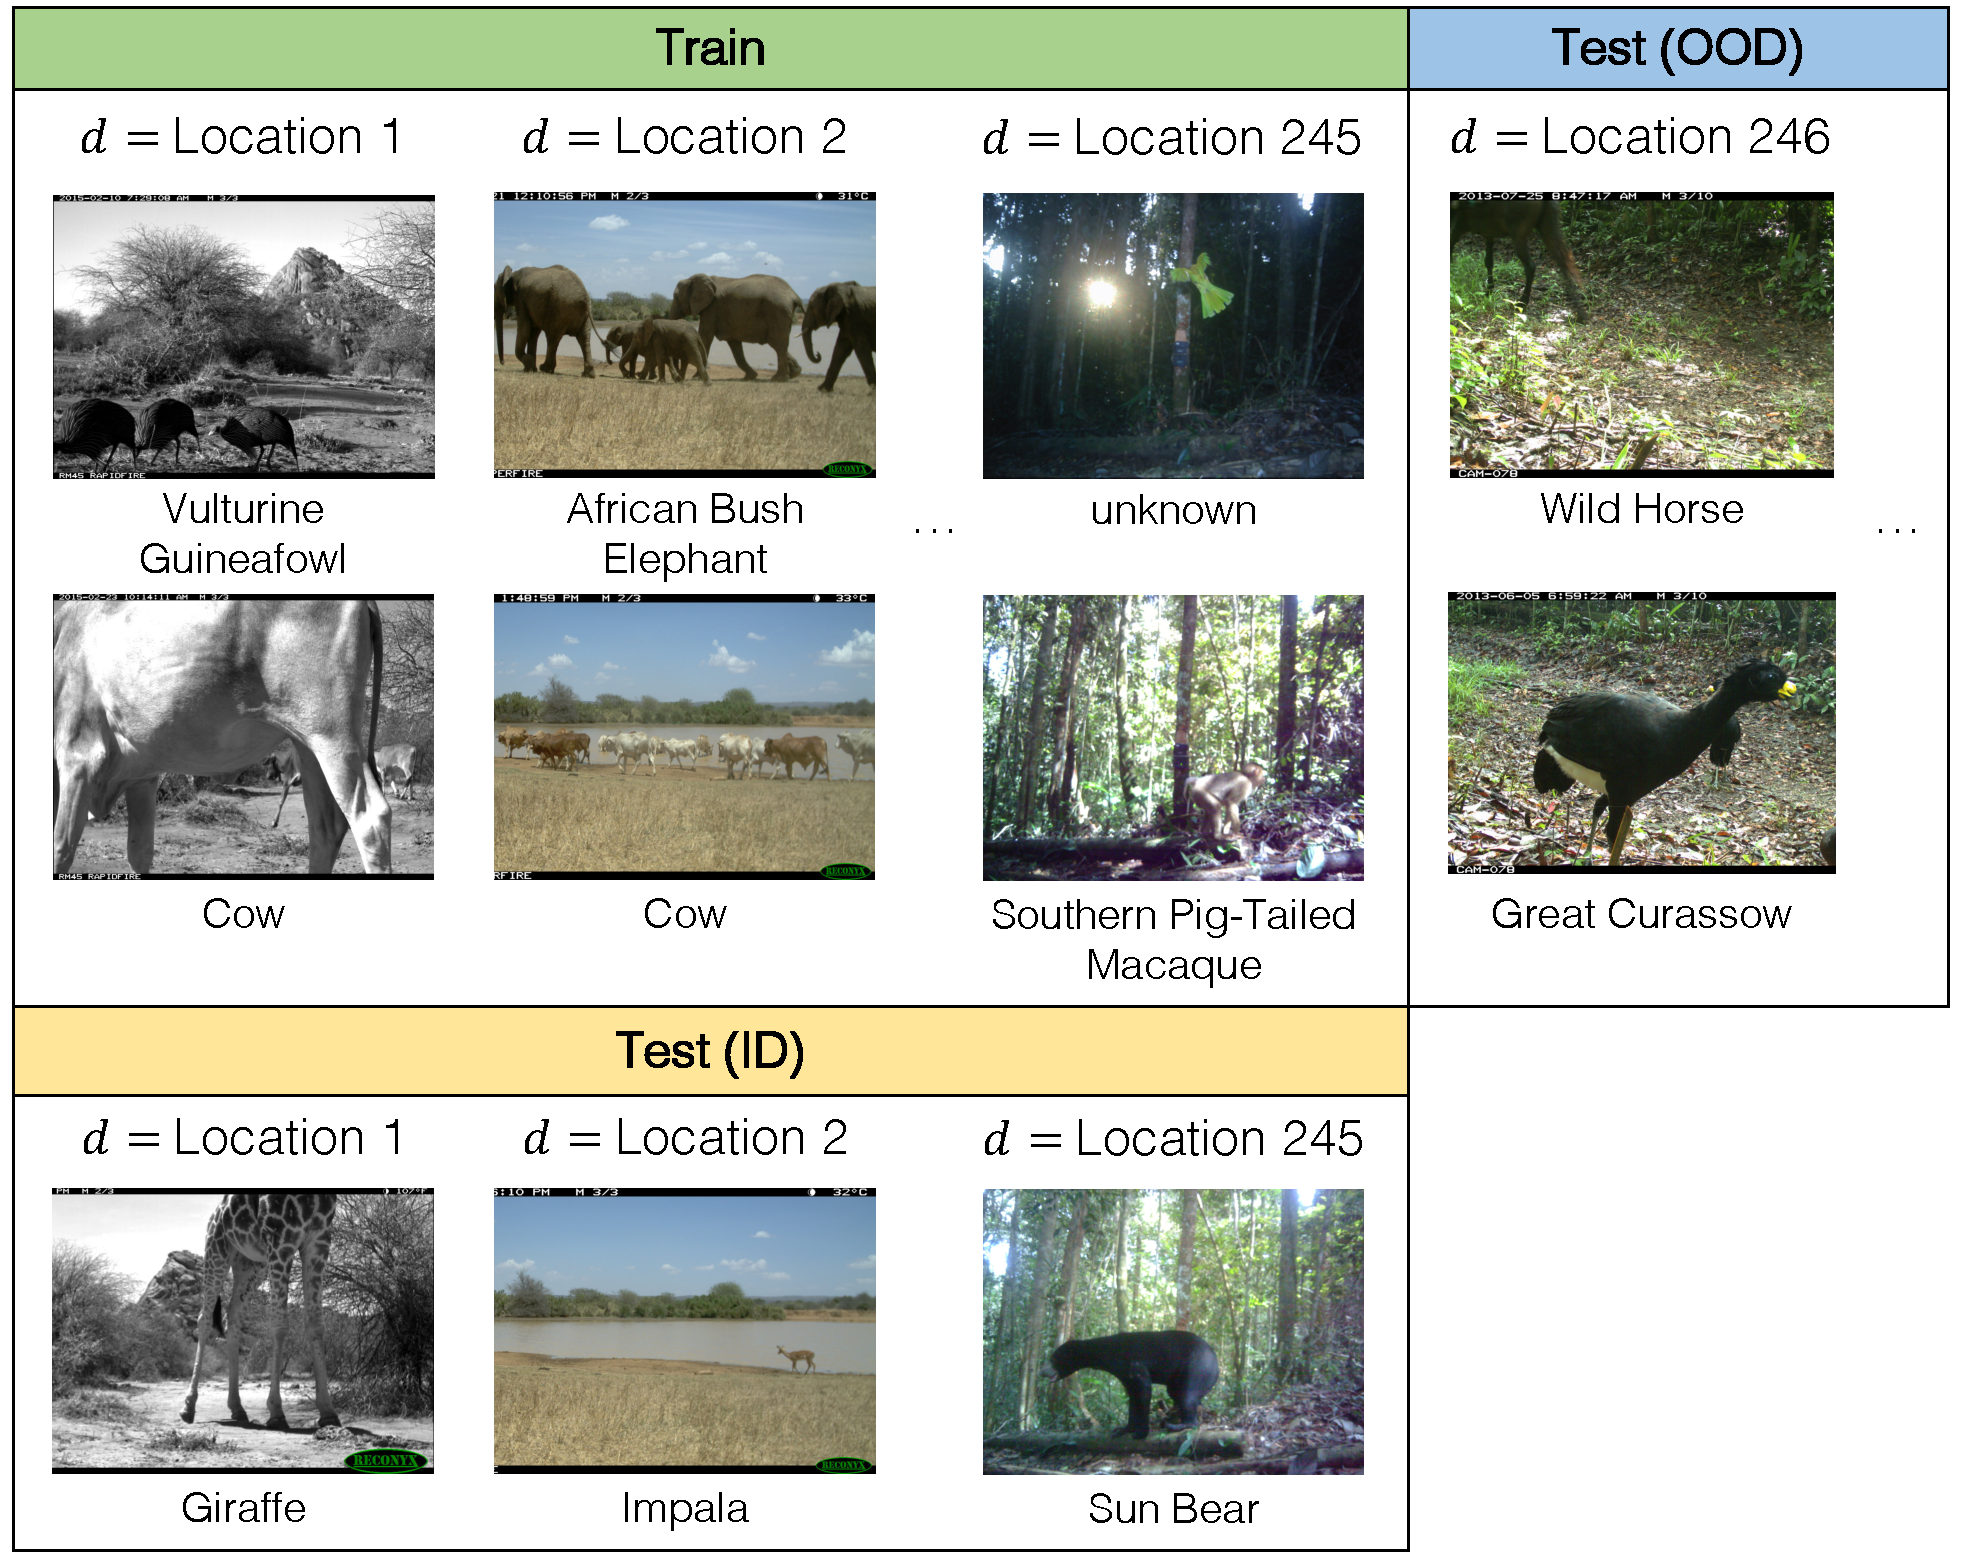
\includegraphics[width=0.85\linewidth]{figures/iwildcam_dataset.pdf}
  \caption{
    The \iWildCam dataset comprises photos of wildlife taken by a variety of camera traps. The goal is to learn models that generalize to photos from new camera traps that are not in the training set.
    Each \Wilds dataset contains both in-distribution (ID) and out-of-distribution (OOD) evaluation sets; for brevity, we omit the ID sets from the subsequent dataset figures.
    }
  \label{fig:dataset_iwildcam}
\end{figure}


Animal populations have declined 68\% on average since 1970 \citep{grooten_peterson_almond}.
To better understand and monitor wildlife biodiversity loss, ecologists commonly deploy camera traps---heat or motion-activated static cameras placed in the wild \citep{wearn2017camera}---and then use ML models to process the data collected \citep{weinstein2018computer,norouzzadeh2019deep,tabak2019machine,beery2019efficient,ahumada2020wildlife}.
Typically, these models would be trained on photos from some existing camera traps and then used across new camera trap deployments.
However, across different camera traps, there is drastic variation in illumination, color, camera angle, background, vegetation, and relative animal frequencies,
which results in models generalizing poorly to new camera trap deployments \citep{beery2018recognition}.

We study this shift on a variant of the iWildCam 2020 dataset \citep{beery2020iwildcam}, where the input $x$ is a photo from a camera trap, the label $y$ is one of 182 animal species, and the domain $d$ specifies the identity of the camera trap (\reffig{dataset_iwildcam}). The training and test sets comprise photos from disjoint sets of camera traps. As leverage, we include over 200 camera traps in the training set, capturing a wide range of variation. We evaluate models by their macro F1 scores, which emphasizes performance on rare species, as rare and endangered species are the most important to accurately monitor.
\refapp{app_iwildcam} provides additional details and context.

\begin{figure}[h!]
  \centering
  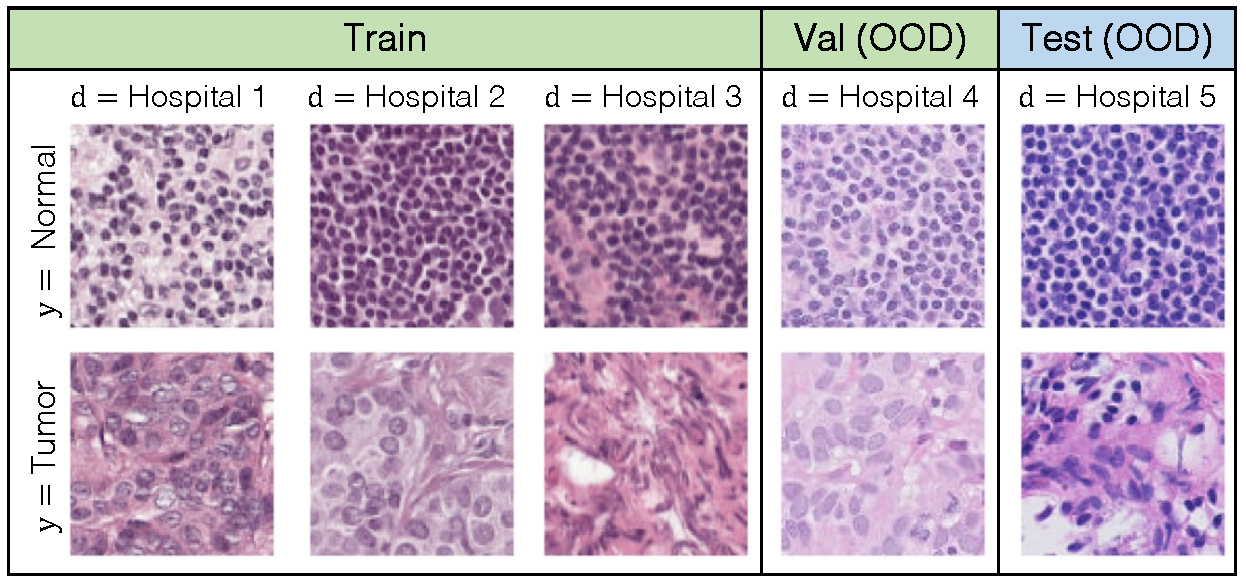
\includegraphics[width=0.85\linewidth]{figures/camelyon_dataset.pdf}
  \caption{
    The \Camelyon dataset comprises tissue patches from different hospitals. The goal is to accurately predict the presence of tumor tissue in patches taken from hospitals that are not in the training set.
    In this figure, each column contains two patches, one of normal tissue and the other of tumor tissue, from the same slide.}
  \label{fig:dataset_camelyon}
\end{figure}

\subsubsection{\Camelyon: Tumor identification across different hospitals}\label{sec:dataset_camelyon}

Models for medical applications are often trained on data from a small number of hospitals, but with the goal of being deployed more generally across other hospitals.
However, variations in data collection and processing can degrade model accuracy on data from new hospital deployments \citep{zech2018radio,albadawy2018tumor}.
In histopathology applications---studying tissue slides under a microscope---this variation can arise from sources like differences in the patient population or in slide staining and image acquisition \citep{veta2016mitosis,komura2018machine,tellez2019quantifying}.

We study this shift on a patch-based variant of the Camelyon17 dataset \citep{bandi2018detection}, where the input $x$ is a 96x96 patch of a whole-slide image of a lymph node section from a patient with potentially metastatic breast cancer, the label $y$ is whether the patch contains tumor, and the domain $d$ specifies which of 5 hospitals the patch was from (\reffig{dataset_camelyon}). The training and test sets comprise class-balanced patches from separate hospitals, and we evaluate models by their average accuracy.
Prior work suggests that staining differences are the main source of variation between hospitals in similar datasets \citep{tellez2019quantifying}. As we have training data from multiple hospitals, a model could use that as leverage to learn to be robust to stain variation.
\refapp{app_camelyon} provides additional details and context.

\subsubsection{\RxRx: Genetic perturbation classification across
experimental batches}\label{sec:dataset_rxrx1}

\begin{figure}[b!]
  \centering
  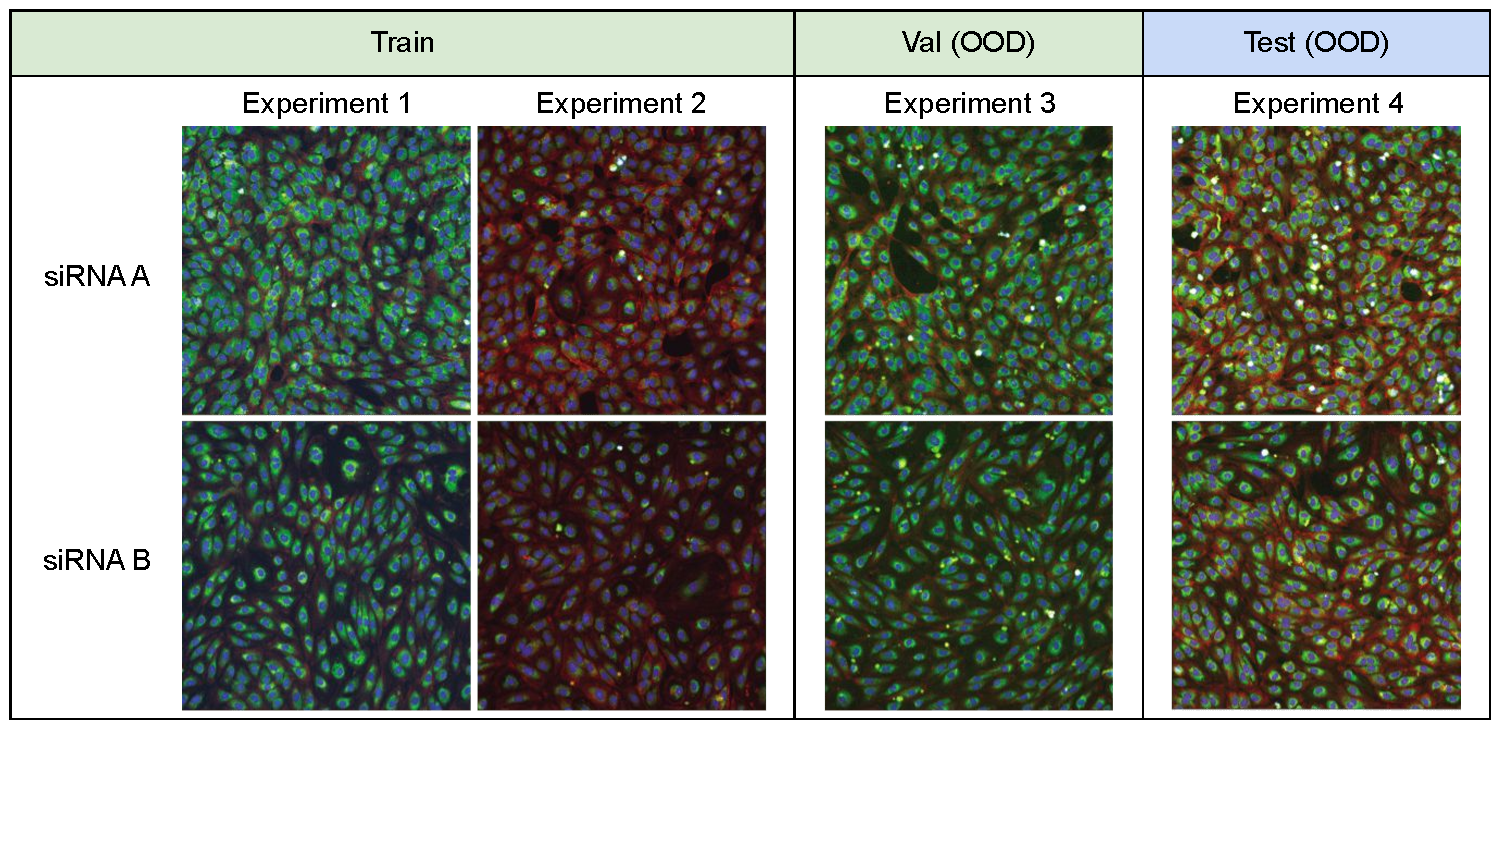
\includegraphics[width=0.85\linewidth]{figures/rxrx1_dataset.pdf}
  \caption{
    The \RxRx dataset comprises images of cells that have been genetically
    perturbed by siRNA~\citep{tuschl2001rna}. The goal is to predict which
    siRNA the cells have been treated with, where the images come from
    experimental batches not in the training set. Here, we show sample
    images from different batches for two of the 1,139 possible classes.}
  \label{fig:dataset_rxrx1}
\end{figure}

High-throughput screening techniques that can generate large amounts of data
are now common in many fields of biology,
including transcriptomics~\citep{harrill2019tox},
genomics~\citep{echeverri2006high,zhou2014high}, proteomics and
metabolomics~\citep{taylor2021spatially}, and drug
discovery~\citep{broach1996high, macarron2011impact, swinney2011were,
boutros2015microscopy}.
Such large volumes of data, however, need to be created in experimental batches, or groups of experiments executed at similar times under similar conditions.
Despite attempts to carefully control experimental variables such as
temperature, humidity, and reagent concentration, measurements from
these screens are confounded by technical artifacts that arise from differences
in the execution of each batch.
These \emph{batch effects} make it difficult to draw conclusions from data  across experimental batches~\citep{leek2010tackling,parker2012practical,soneson2014batch,nygaard2016methods,caicedo2017data}.

We study the shift induced by batch effects on a variant of the RxRx1
dataset~\citep{taylor2019rxrx1}, where the input $x$ is a 3-channel image of
cells obtained by fluorescent microscopy \citep{bray2016cell}, the label $y$
indicates which of the 1,139 genetic treatments (including no treatment) the
cells received, and the domain $d$ specifies the batch in which the imaging
experiment was run.
As summarized in \reffig{dataset_rxrx1}, the training and test sets consist of disjoint experimental batches.
As leverage, the training set has images from 33 different batches, with each batch containing one sample for every class.
We assess a model's ability to normalize
batch effects while preserving biological signal by evaluating how well it can
classify images of treated cells in the out-of-distribution test set.
\refapp{app_rxrx1} provides additional details and context.

\subsubsection{\Mol: Molecular property prediction across different scaffolds}\label{sec:dataset_molpcba}

Accurate prediction of the biochemical properties of small molecules can  significantly accelerate drug discovery by reducing the need for expensive lab experiments \citep{shoichet2004virtual,hughes2011principles}.
However, the experimental data available for training such models is limited compared to the extremely diverse and combinatorially large universe of candidate molecules that we would want to make predictions on \citep{bohacek1996art,sterling2015,lyu2019ultra,mccloskey2020machine}.
This means that models need to generalize to out-of-distribution molecules that are structurally different from those seen in the training set.

We study this shift on the \Mol dataset, which is directly adopted from the Open Graph Benchmark~\citep{hu2020open} and originally from MoleculeNet~\citep{wu2018moleculenet}. As summarized in \reffig{dataset_molpcba}, it is a multi-label classification dataset, where the input $x$ is a molecular graph, the label $y$ is a 128-dimensional binary vector where each component corresponds to a biochemical assay result, and the domain $d$ specifies the scaffold (i.e., a cluster of molecules with similar structure). The training and test sets comprise molecules with disjoint scaffolds; for leverage, the training set has molecules from over 40,000 scaffolds. We evaluate models by averaging the Average Precision (AP) across each of the 128 assays.
\refapp{app_molpcba} provides additional details and context.

\begin{figure}[h!]
  \centering
  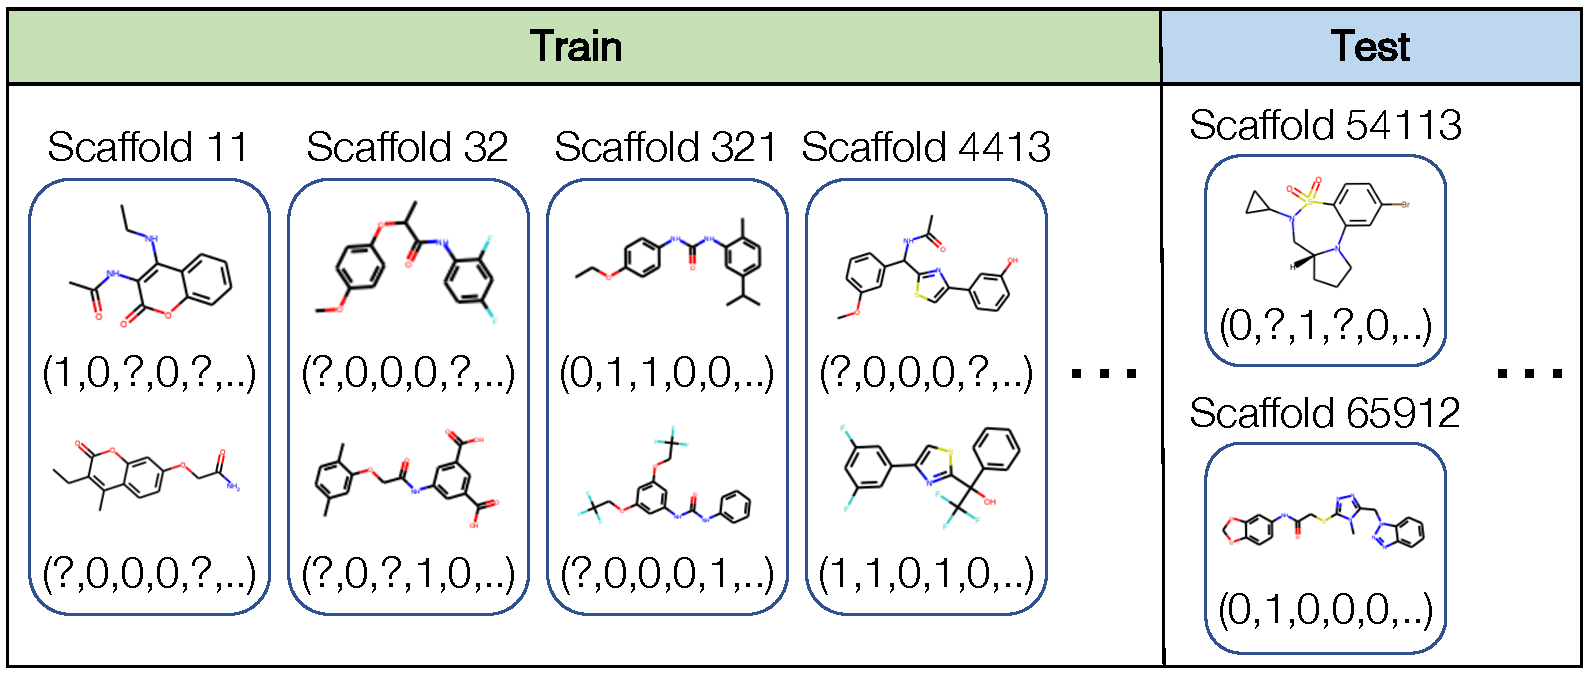
\includegraphics[width=0.9\linewidth]{figures/molpcba_dataset.pdf}
  \caption{
    The \Mol dataset comprises molecules with many different structural scaffolds. The goal is to predict biochemical assay results in molecules with scaffolds that are not in the training set. Here, we show sample molecules from each scaffold, together with target labels: each molecule is associated with 128 binary labels and `?' indicates that the label is not provided for the molecule.}
  \label{fig:dataset_molpcba}
\end{figure}


\subsubsection{\Wheat: Wheat head detection across regions of the world}\label{sec:dataset_wheat}

Models for automated, high-throughput plant phenotyping---measuring the physical characteristics of plants and crops, such as wheat head density and counts---are important tools for crop breeding \citep{thorp2018high,reynolds2020breeder} and agricultural field management~\citep{shi2016uav}.
These models are typically trained on data collected in a limited number of regions, even for crops grown worldwide such as wheat \citep{madec2019ear, xiong2019tasselnetv2,ubbens2020autocount, ayalew2020unsupervised}.
However, there can be substantial variation between regions, due to differences in crop varieties, growing conditions, and data collection protocols.
Prior work on wheat head detection has shown that this variation can significantly degrade model performance on regions unseen during training \citep{david2020global}.

We study this shift in an expanded version of the Global Wheat Head Dataset~\citep{david2020global,david2021global}, a large set of wheat images collected from 12 countries around the world (\reffig{dataset_wheat}).
It is a detection dataset, where the input $x$ is a cropped overhead image of a wheat field, the label $y$ is the set of bounding boxes for each wheat head visible in the image, and the domain $d$ specifies an image acquisition session (i.e., a specific location, time, and sensor with which a set of images was collected).
The data split captures a shift in location, with training and test sets comprising images from disjoint countries.
As leverage, we include images from 18 acquisition sessions over 5 countries in the training set.
We evaluate model performance on unseen countries by measuring accuracy at a fixed Intersection over Union (IoU) threshold, and averaging across acquisition sessions to account for imbalances in the numbers of images in them.
Additional details are provided in \refapp{app_wheat}.

\begin{figure}[h!]
  \centering
  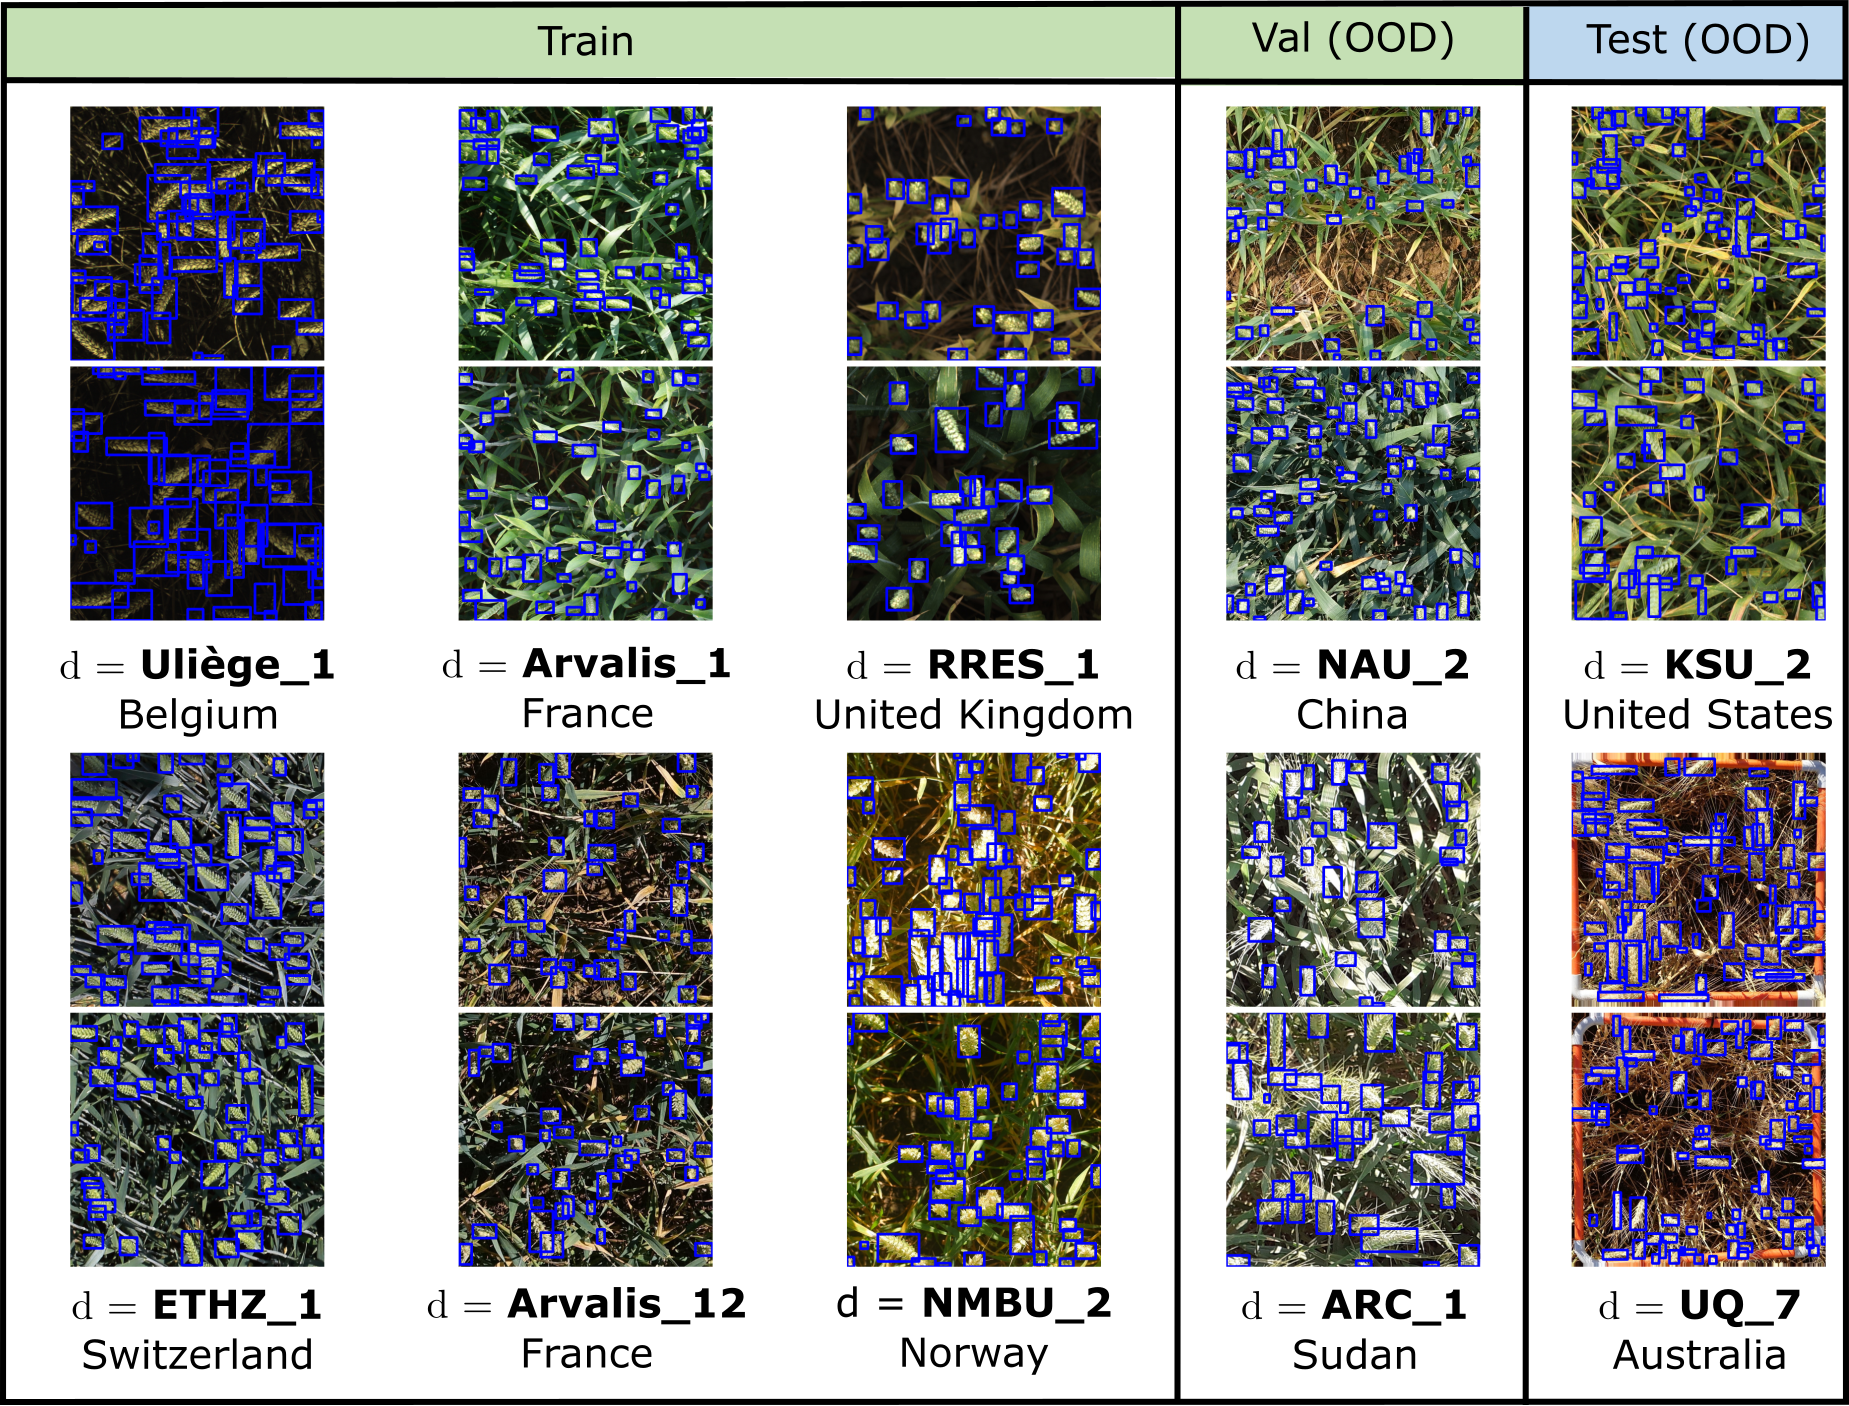
\includegraphics[width=0.9\linewidth]{figures/wheat_dataset.png}
  \caption{
    The \Wheat dataset consists of overhead images of wheat fields, annotated with bounding boxes of wheat heads. The goal is to detect and predict the bounding boxes of wheat heads, where images are from new acquisition sessions. A set of wheat images are collected in each acquisition session, each corresponding to a specific wheat field location, time, and sensor. While acquisition sessions vary along multiple axes, from the aforementioned factors to wheat growth stage to illumination conditions, the dataset split primarily captures a shift in location; test images are taken from countries unseen during training time. In this figure, we show images with bounding boxes from different acquisition sessions.
    }
  \label{fig:dataset_wheat}
\end{figure}


\subsection{Subpopulation shift datasets}

\subsubsection{\CivilComments: Toxicity classification across demographic identities}\label{sec:dataset_civilcomments}

Automatic review of user-generated text is an important tool for moderating the sheer volume of text written on the Internet.
We focus here on the task of detecting toxic comments.
Prior work has shown that toxicity classifiers can pick up on biases in the training data and spuriously associate toxicity with the mention of certain demographics \citep{park2018reducing, dixon2018measuring}.
These types of spurious correlations can significantly degrade model performance on particular subpopulations \citep{sagawa2020group}.

We study this problem on a variant of the CivilComments dataset \citep{borkan2019nuanced}, a large collection of comments on online articles taken from the Civil Comments platform (\reffig{dataset_civilcomments}).
The input $x$ is a text comment, the label $y$ is whether the comment was rated as toxic, and the domain $d$ is a 8-dimensional binary vector where each component corresponds to whether the comment mentions one of the 8 demographic identities \textit{male}, \textit{female}, \textit{LGBTQ}, \textit{Christian}, \textit{Muslim}, \textit{other religions}, \textit{Black}, and \textit{White}.
The training and test sets comprise comments on disjoint articles, and we evaluate models by the lowest true positive/negative rate over each of these 8 demographic groups; these groups overlap with each other, deviating slightly from the standard subpopulation shift framework in \refsec{problems}.
Models can use the provided domain annotations as leverage to learn to perform well over each demographic group.
\refapp{app_civilcomments} provides additional details and context.

\begin{figure}[!h]
  \centering
  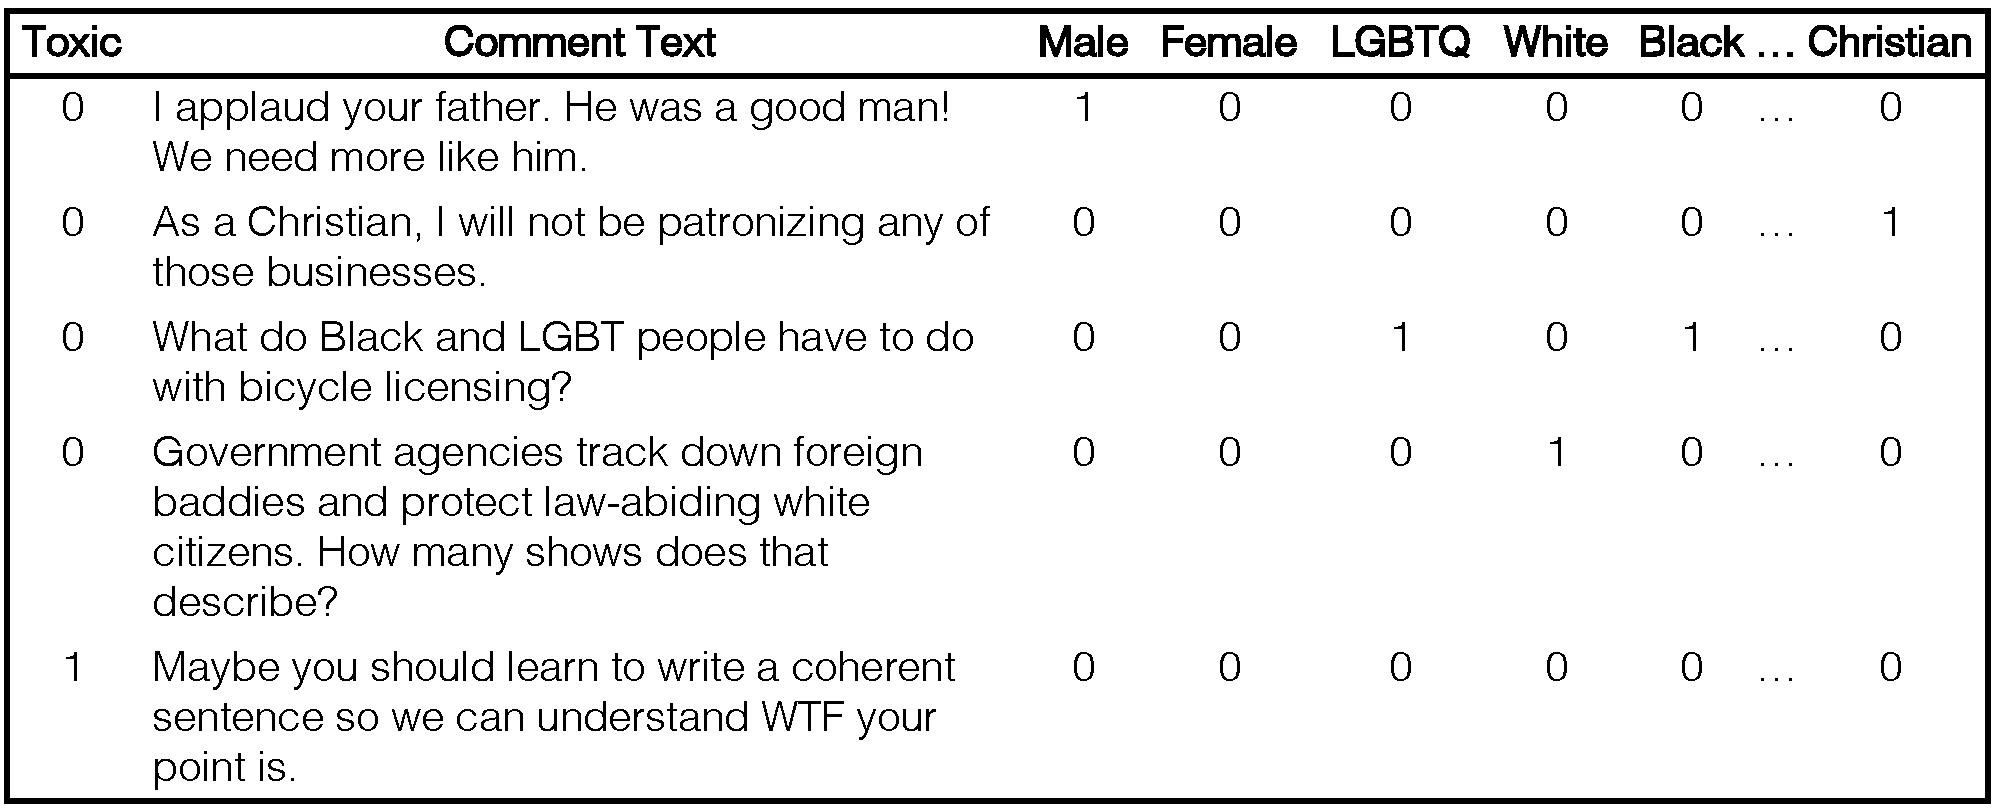
\includegraphics[width=0.9\linewidth]{figures/civilcomments_dataset.pdf}
  \caption{
    The \CivilComments dataset involves classifying the toxicity of online comments. The goal is to learn models that avoid spuriously associating mentions of demographic identities (like male, female, etc.) with toxicity due to biases in the training data.
    }
  \label{fig:dataset_civilcomments}
\end{figure}

\subsection{Hybrid datasets}

\subsubsection{\FMoW: Land use classification across different regions and years}\label{sec:dataset_fmow}
ML models for satellite imagery can enable global-scale monitoring of sustainability and economic challenges, aiding policy and humanitarian efforts in applications such as deforestation tracking~\citep{hansen2013forest}, population density mapping~\citep{tiecke2017population}, crop yield prediction~\citep{wang2020weakly}, and other economic tracking applications~\citep{katona2018parking}.
As satellite data constantly changes due to human activity and environmental processes, these models must be robust to distribution shifts over time.
Moreover, as there can be disparities in the data available between regions,
these models should ideally have uniformly high accuracies instead of only doing well on data-rich regions and countries.

We study this problem on a variant of the Functional Map of the World dataset \citep{christie2018fmow}, where the input $x$ is an RGB satellite image, the label $y$ is one of 62 building or land use categories, and the domain $d$ represents the year the image was taken and its geographical region (Africa, the Americas, Oceania, Asia, or Europe) (\reffig{dataset_fmow}). The different regions have different numbers of examples, e.g., there are far fewer images from Africa than the Americas.
The training set comprises data from before 2013, while the test set comprises data from 2016 and after; years 2013 to 2015 are reserved for the validation set.
We evaluate models by their test accuracy on the worst geographical region, which combines both a domain generalization problem over time and a subpopulation shift problem over regions.
As we provide both time and region annotations, models can leverage the structure across both space and time to improve robustness.
\refapp{app_fmow} provides additional details and context.

\begin{figure}[!t]
  \centering
  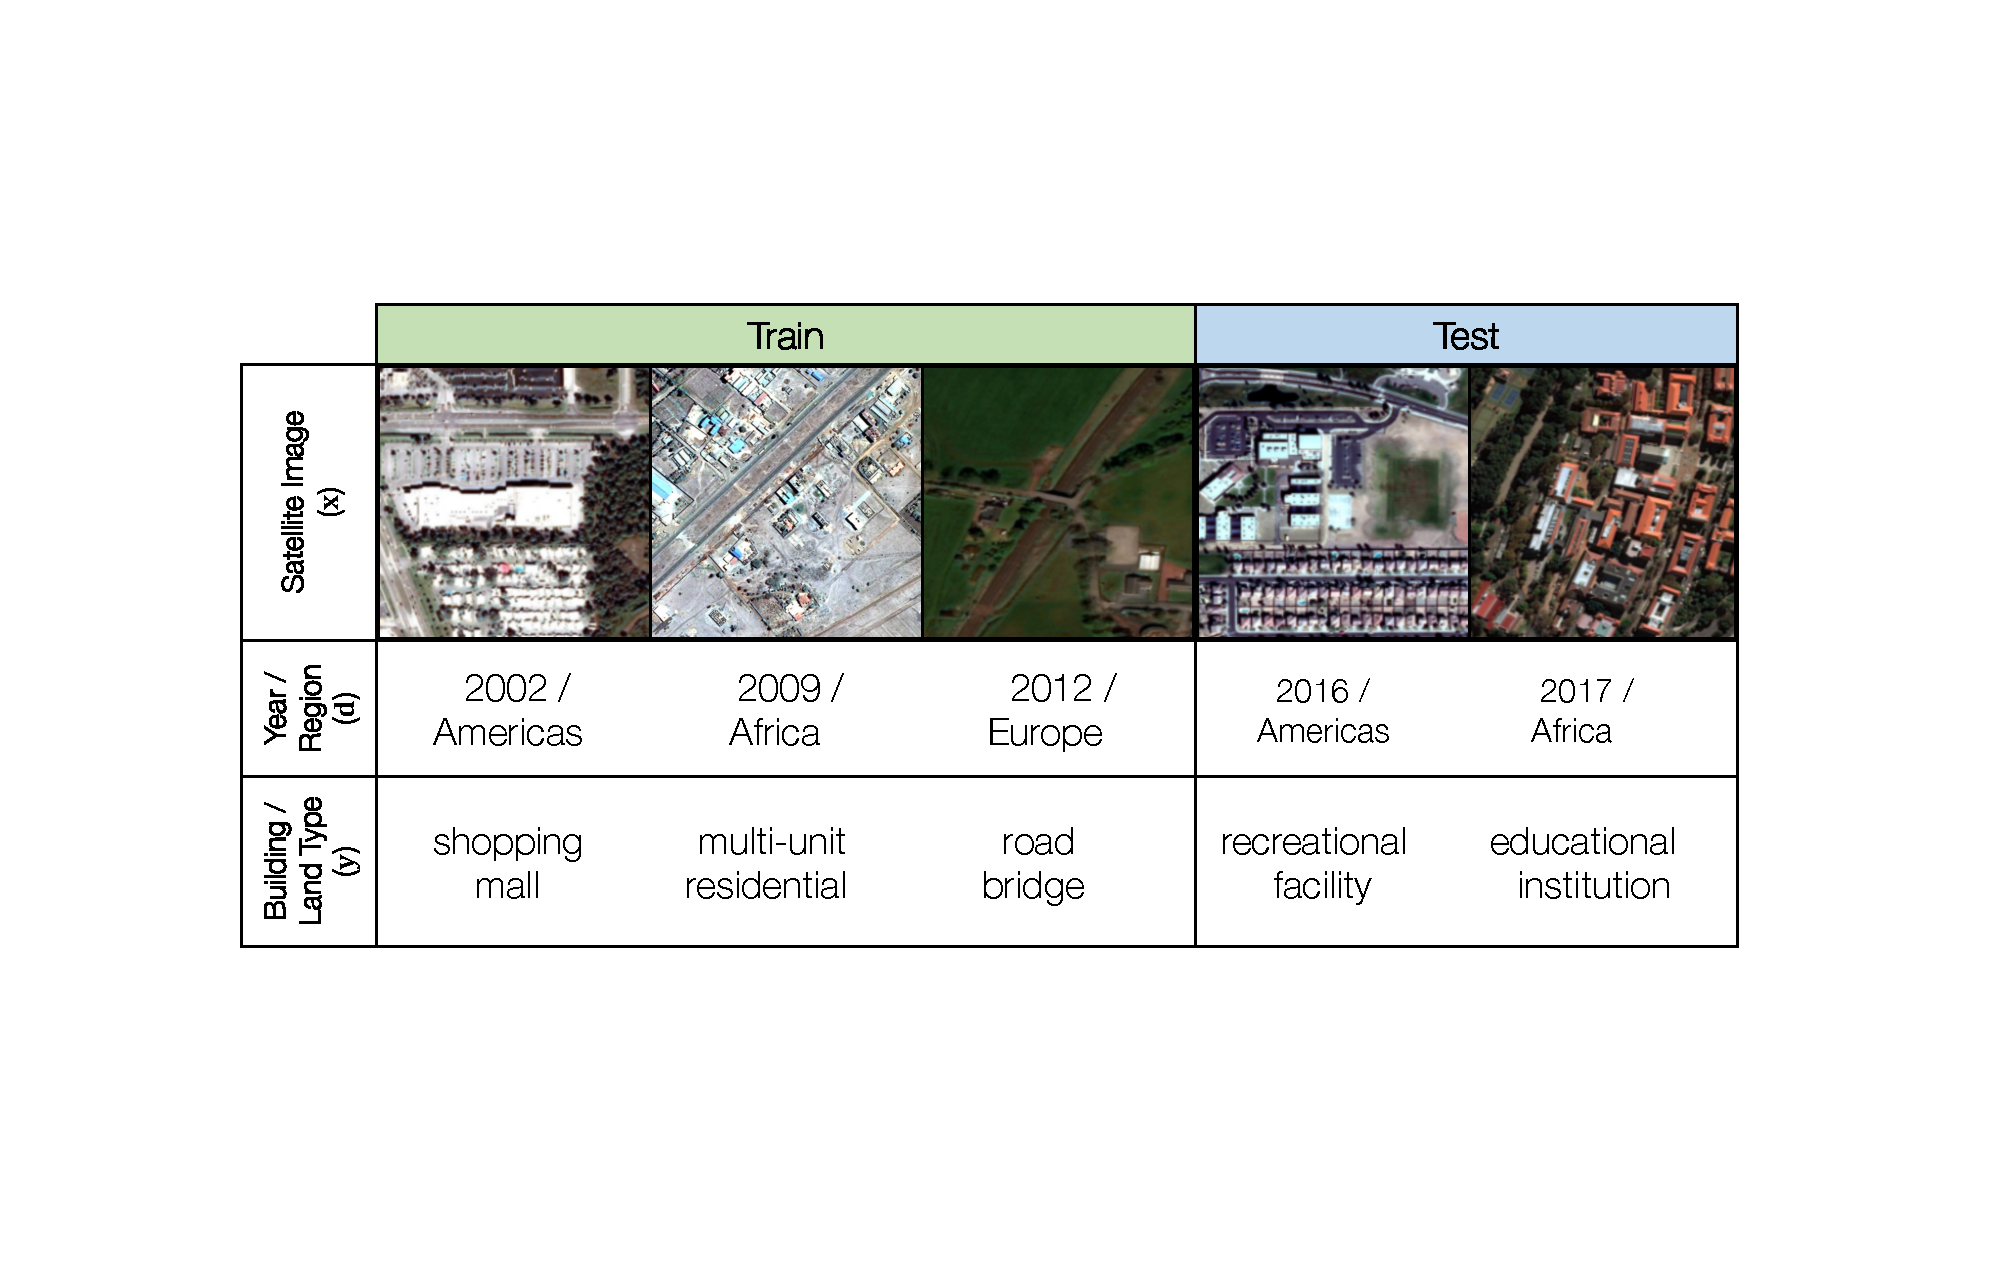
\includegraphics[width=0.9\linewidth]{figures/fmow_dataset.pdf}
  \caption{
  The \FMoW dataset contains satellite images taken in different geographical regions and at different times. The goal is to generalize to satellite imagery taken in the future, which may be shifted due to infrastructure development across time, and to do equally well across geographic regions.
  }\label{fig:dataset_fmow}
\end{figure}

\subsubsection{\PovertyMap: Poverty mapping across different countries}\label{sec:dataset_povertymap}

Global-scale poverty estimation is a specific remote sensing application which is essential for targeted humanitarian efforts in poor regions \citep{abelson2014poor,epsey2015development}.
However, ground truth measurements of poverty are lacking for much of the developing world, as field surveys for collecting the ground truth are expensive~\citep{blumenstock2015poverty}.
This motivates the approach of training ML models on countries with ground truth labels and then deploying them on different countries where we have satellite data but no labels \citep{xie2016transfer,jean2016combining,yeh2020poverty}.

We study this shift through a variant of the poverty mapping dataset collected by \citet{yeh2020poverty}, where the input $x$ is a multispectral satellite image, the output $y$ is a real-valued asset wealth index from surveys, and the domain $d$ represents the country the image was taken in and whether the image is of an urban or rural area (\reffig{dataset_poverty}). The training and test set comprise data from disjoint sets of countries, and we evaluate models by the correlation of their predictions with the ground truth. Specifically, we take the lower of the correlations over the urban and rural subpopulations, as prior work has shown that accurately predicting poverty within these subpopulations is especially challenging.
As poverty measures are highly correlated across space \citep{jean2018ssdkl,rolf2020post}, methods can utilize the provided location coordinates, and the country and urban/rural annotations, to improve robustness.
\refapp{app_povertymap} provides additional details and context.

\begin{figure}[h!]
  \centering
  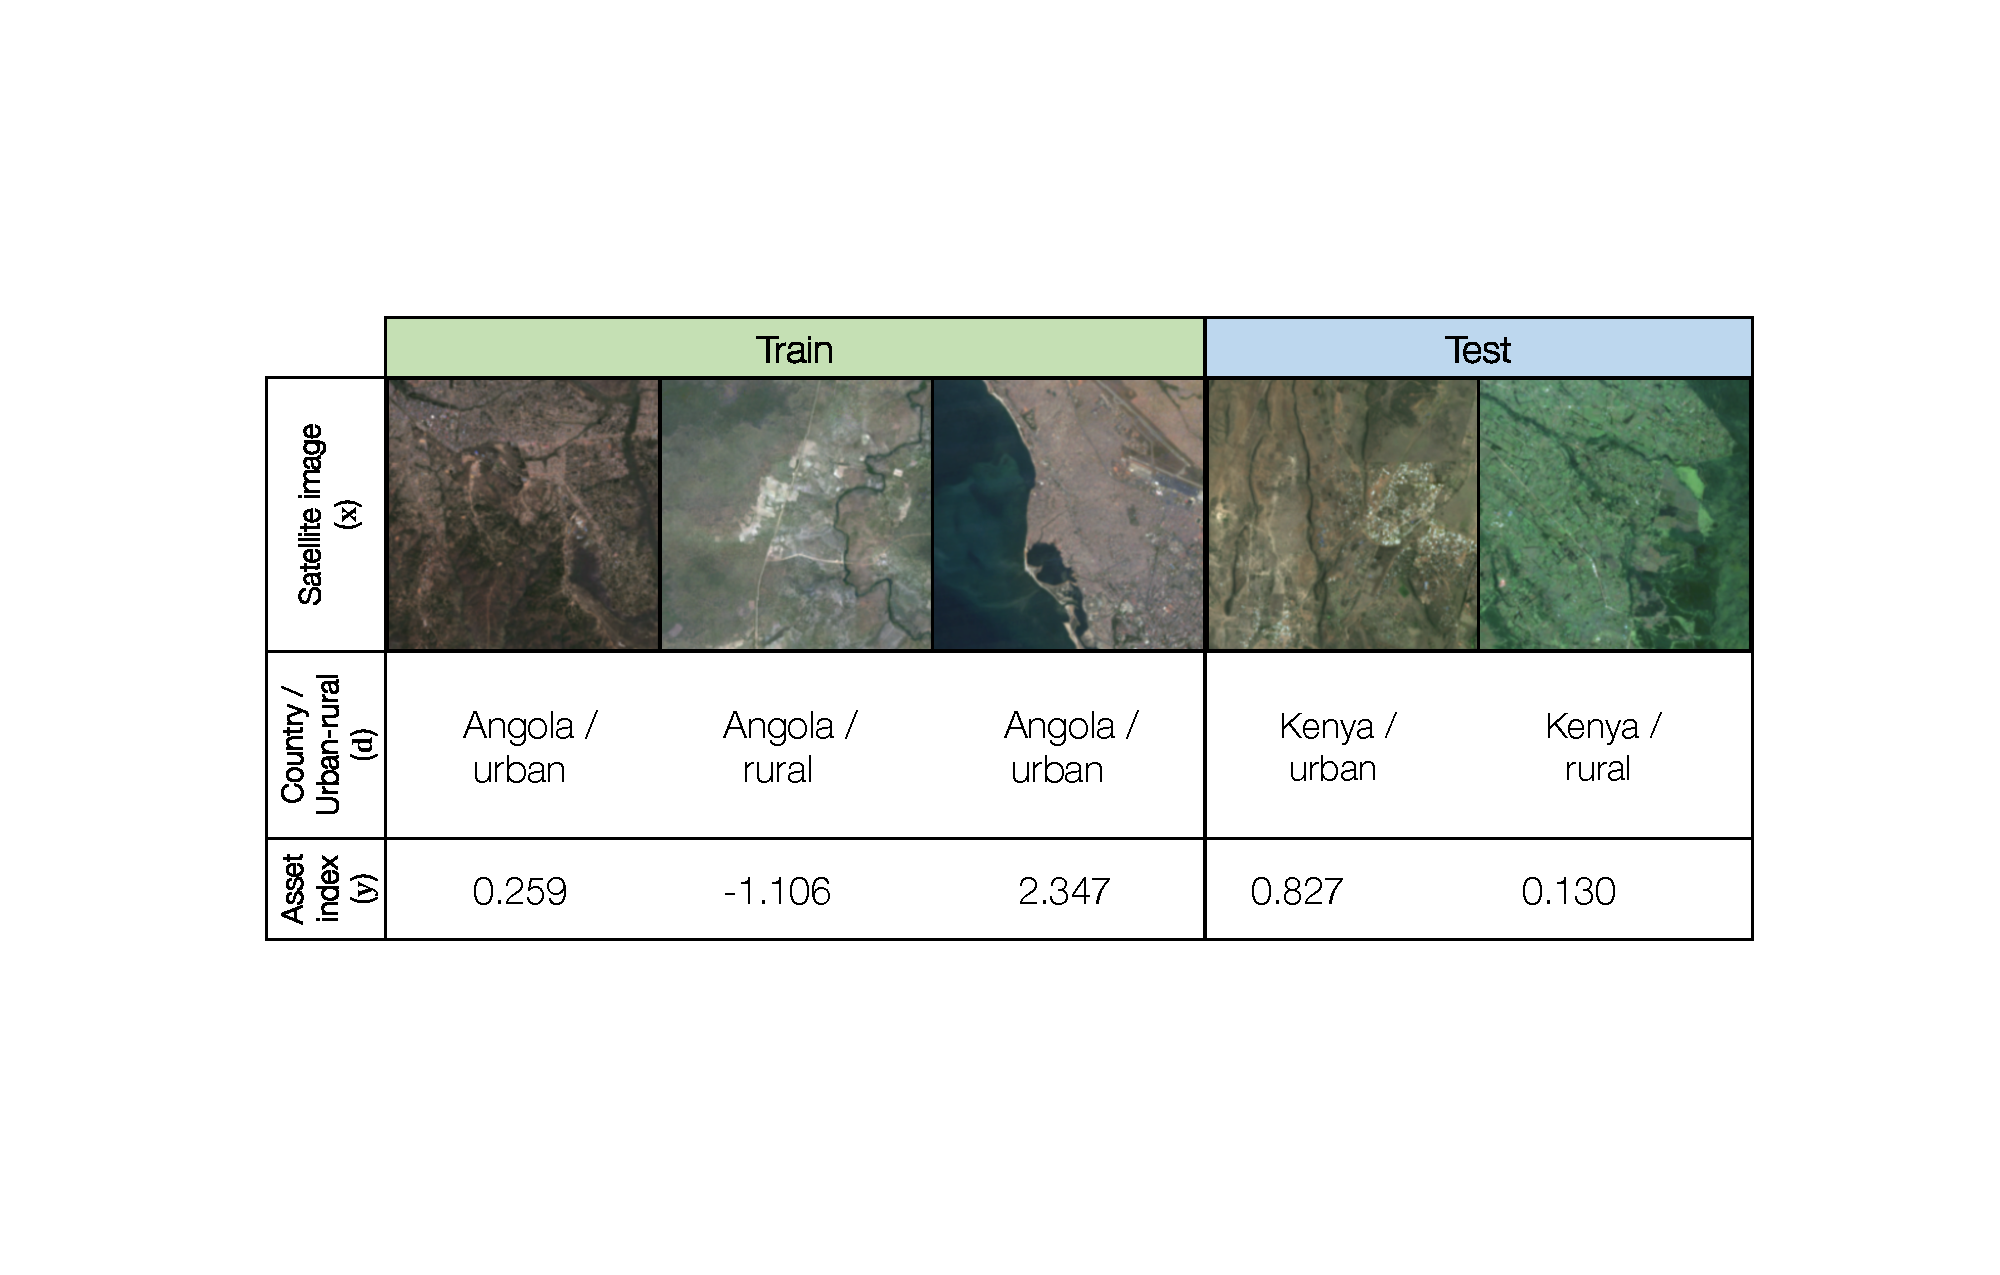
\includegraphics[width=0.9\linewidth]{figures/poverty_dataset.pdf}
  \caption{The \PovertyMap dataset contains satellite images taken in different countries. The goal is to predict asset wealth in countries that are not present in the training set, while being accurate in both urban and rural areas. There may be significant economic and cultural differences across country borders that contribute to the spatial distribution shift.}\label{fig:dataset_poverty}
\end{figure}


\begin{figure}[h!]
  \centering
  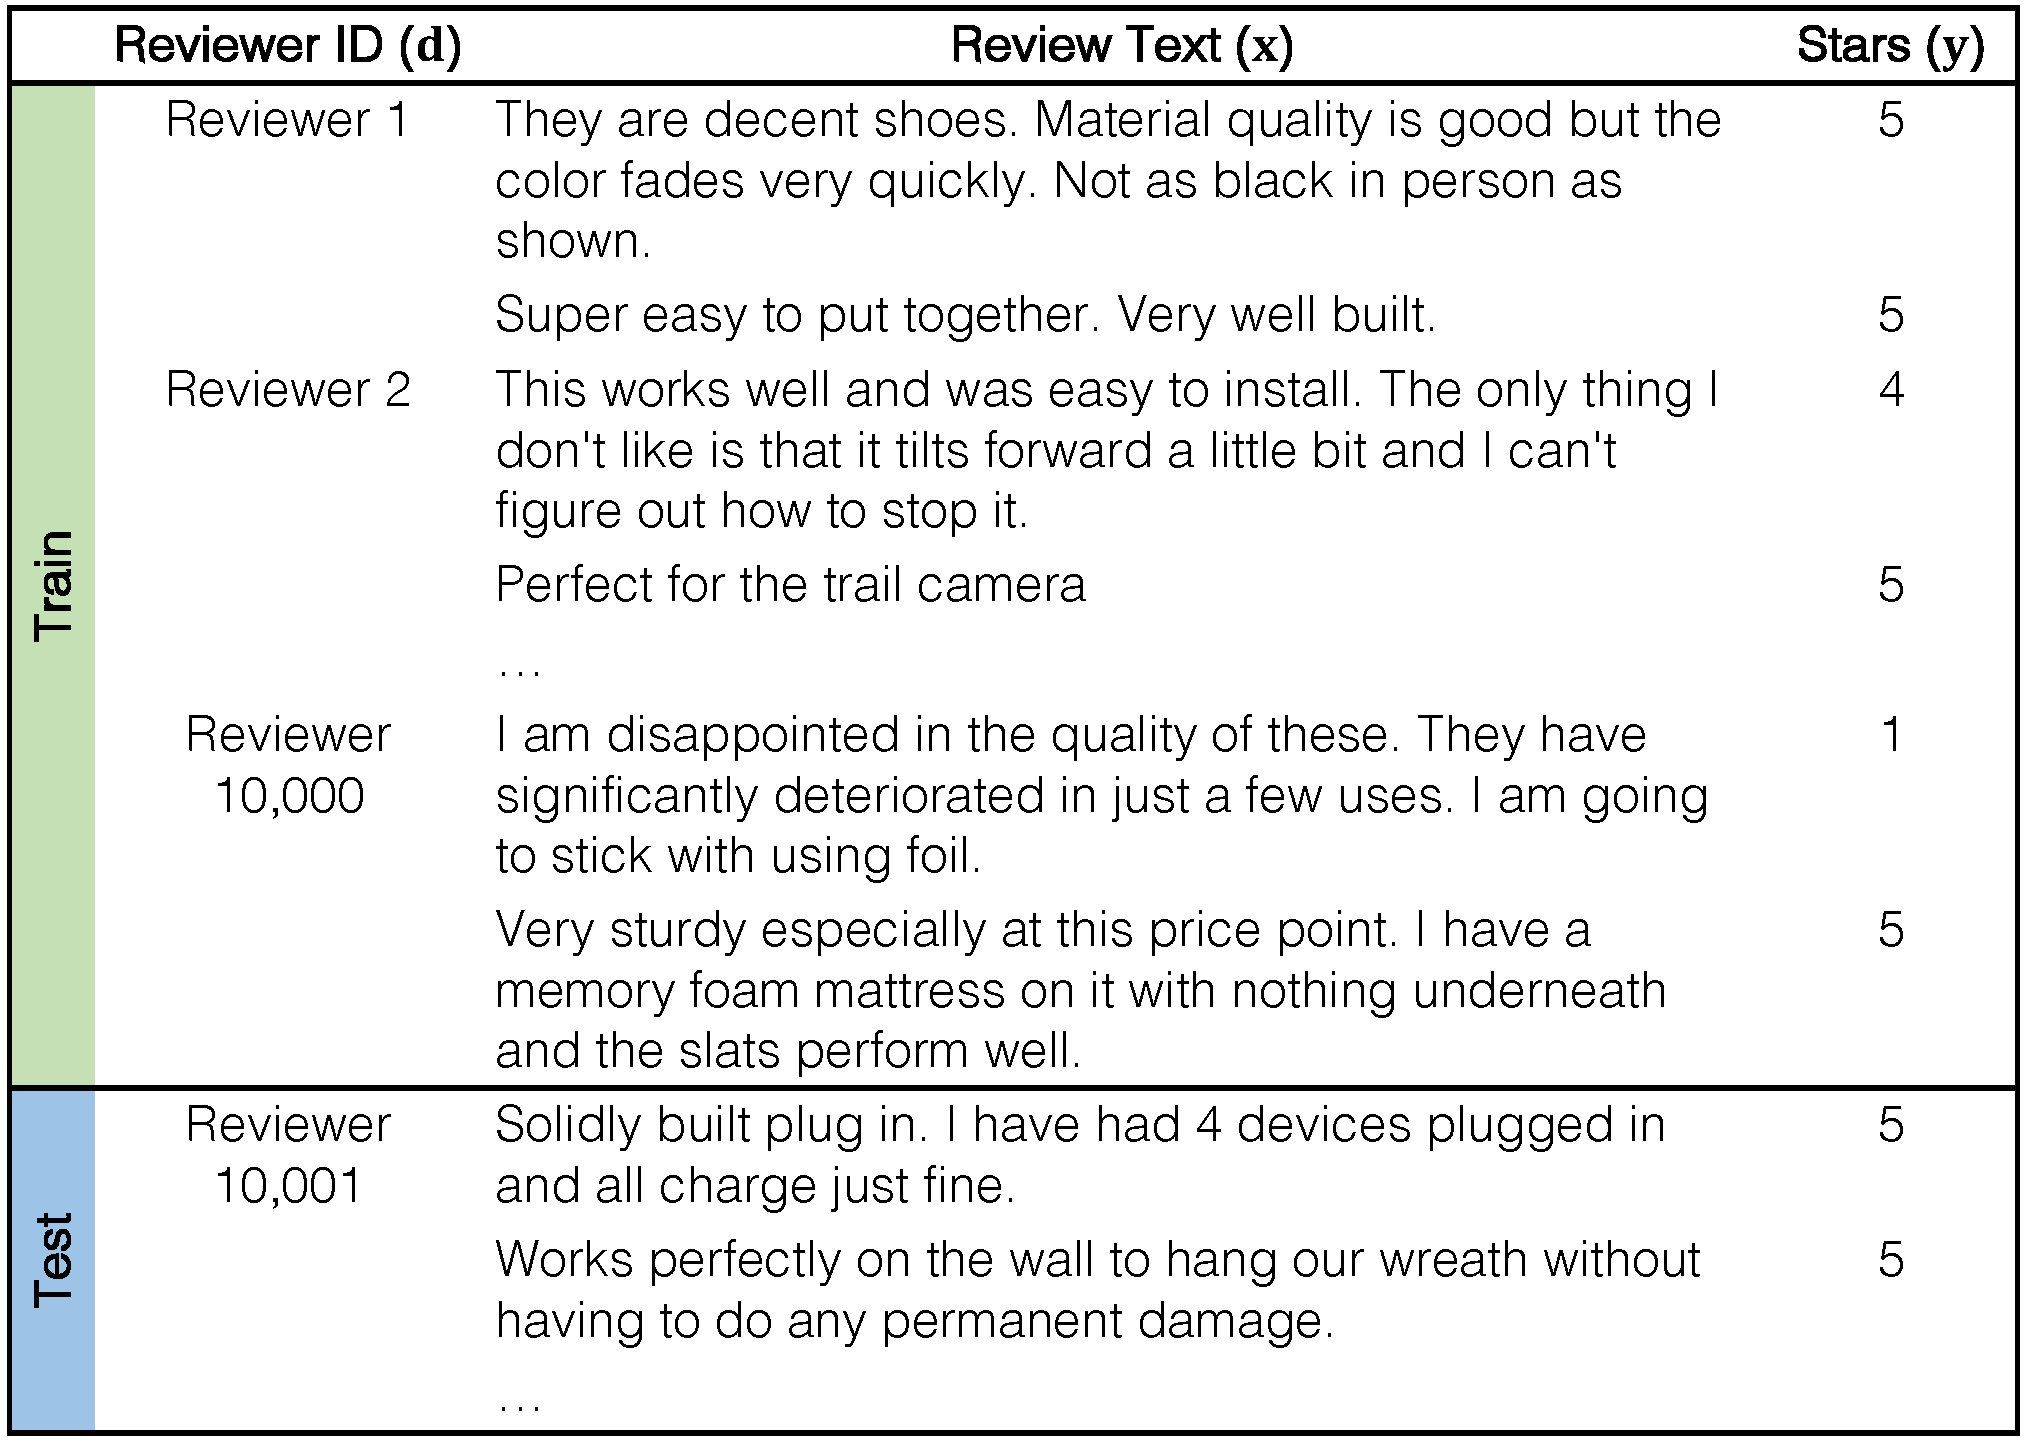
\includegraphics[width=0.75\linewidth]{figures/amazon_dataset.pdf}
  \caption{
    The \Amazon dataset involves predicting star ratings from reviews of Amazon products. The goal is to do consistently well on new reviewers who are not in the training set.
    }
  \label{fig:dataset_amazon}
\end{figure}

\subsubsection{\Amazon: Sentiment classification across different users}\label{sec:dataset_amazon}

In many consumer-facing ML applications, models are trained on data collected on one set of users and then deployed across a wide range of potentially new users.
These models can perform well on average but poorly on some users \citep{tatman2017,caldas2018leaf,li2019fair,koenecke2020racial}.
These large performance disparities across users are practical concerns in consumer-facing applications, and they can also indicate that models are exploiting biases or spurious correlations in the data \citep{badgeley2019deep,geva2019annotator}.

We study this issue on a variant of the Amazon review dataset \citep{ni2019justifying}, where the input $x$ is the review text, the label $y$ is the corresponding 1-to-5 star rating, and the domain $d$ identifies the user who wrote the review (\reffig{dataset_amazon}). The training and test sets comprise reviews from disjoint sets of users; for leverage, the training set has reviews from 5,008 different users. As our goal is to train models with consistently high performance across users, we evaluate models by the 10th percentile of per-user accuracies.
\refapp{app_amazon} provides additional details and context.
We discuss other distribution shifts on this dataset (e.g., by category) in \refapp{app_amazon_other}.


\subsubsection{\Py: Code completion across different codebases}\label{sec:dataset_py150}

Code completion models---autocomplete tools used by programmers to suggest subsequent source code tokens, such as the names of API calls---are commonly used to reduce the effort of software development \citep{robbes2008program,bruch2009learning,nguyen2015graph,proksch2015intelligent,franks2015cacheca}.
These models are typically trained on data collected from existing codebases but then deployed more generally across other codebases, which may have different distributions of API usages \citep{nita2010using,proksch2016evaluating,allamanis2017smartpaste}.
This shift across codebases can cause substantial performance drops in code completion models.
Moreover, prior studies of real-world usage of code completion models have noted that they can generalize poorly on some important subpopulations of tokens such as method names \citep{hellendoorn2019code}.

We study a variant of the Py150 Dataset \citep{raychev2016probabilistic,CodeXGLUE}, where the goal is to predict the next token (e.g., \texttt{"environ"}, \texttt{"communicate"} in \reffig{dataset_py150}) given the context of previous tokens.
The input $x$ is a sequence of source code tokens, the label $y$ is the next token, and the domain $d$ specifies the repository that the source code belongs to.
The training and test sets comprise code from disjoint GitHub repositories.
As leverage, we include over 5,300 repositories in the training set, capturing a wide range of source code variation. We evaluate models by their accuracy on the subpopulation of class and method tokens.
Additional dataset and model details are provided in \refapp{app_py150}.

\begin{figure}[h]
  \centering
  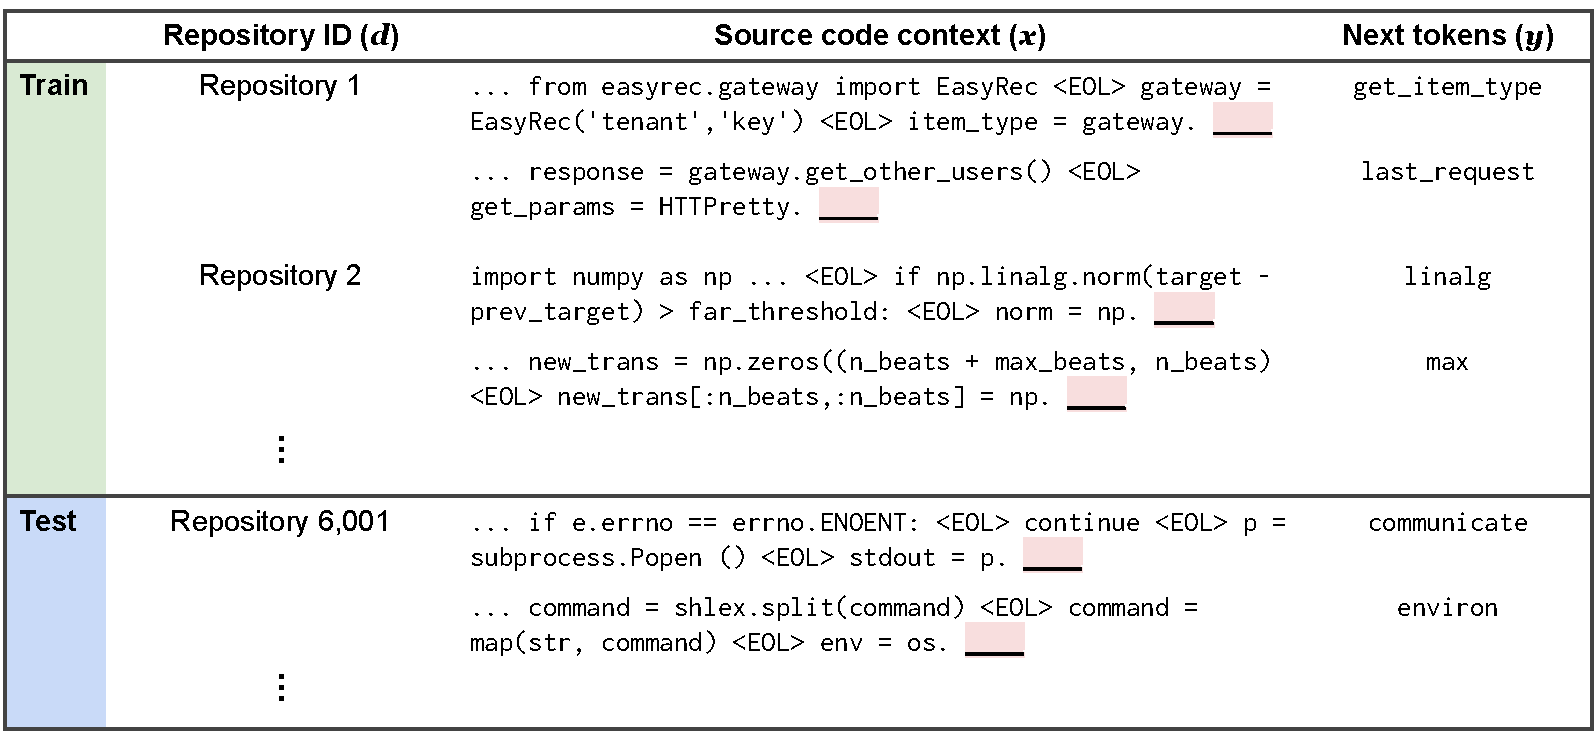
\includegraphics[width=1.0\linewidth]{figures/py150_dataset.pdf}
  \caption{
    The \Py dataset comprises Python source code files taken from a variety of public repositories on GitHub. The task is code completion: predict token names given the context of previous tokens. We evaluate models on their accuracy on the subpopulation of API calls (i.e., method and class tokens), which are the most common code completion queries in real-world settings. Our goal is to learn code completion models that generalize to source code in new repositories that are not seen in the training set.
    }
  \label{fig:dataset_py150}
\end{figure}
